% ---- SECTION MATÉRIELS ET MÉTHODES ----

% -------------------------------------------------------
\section{Architecture système globale}
% -------------------------------------------------------
Le système \textbf{SMART-SOJA} repose sur une architecture modulaire et hiérarchisée structurée en trois couches fonctionnelles (Figure \ref{fig:architecture_complete}) :

\begin{figure}[H]
    \centering
    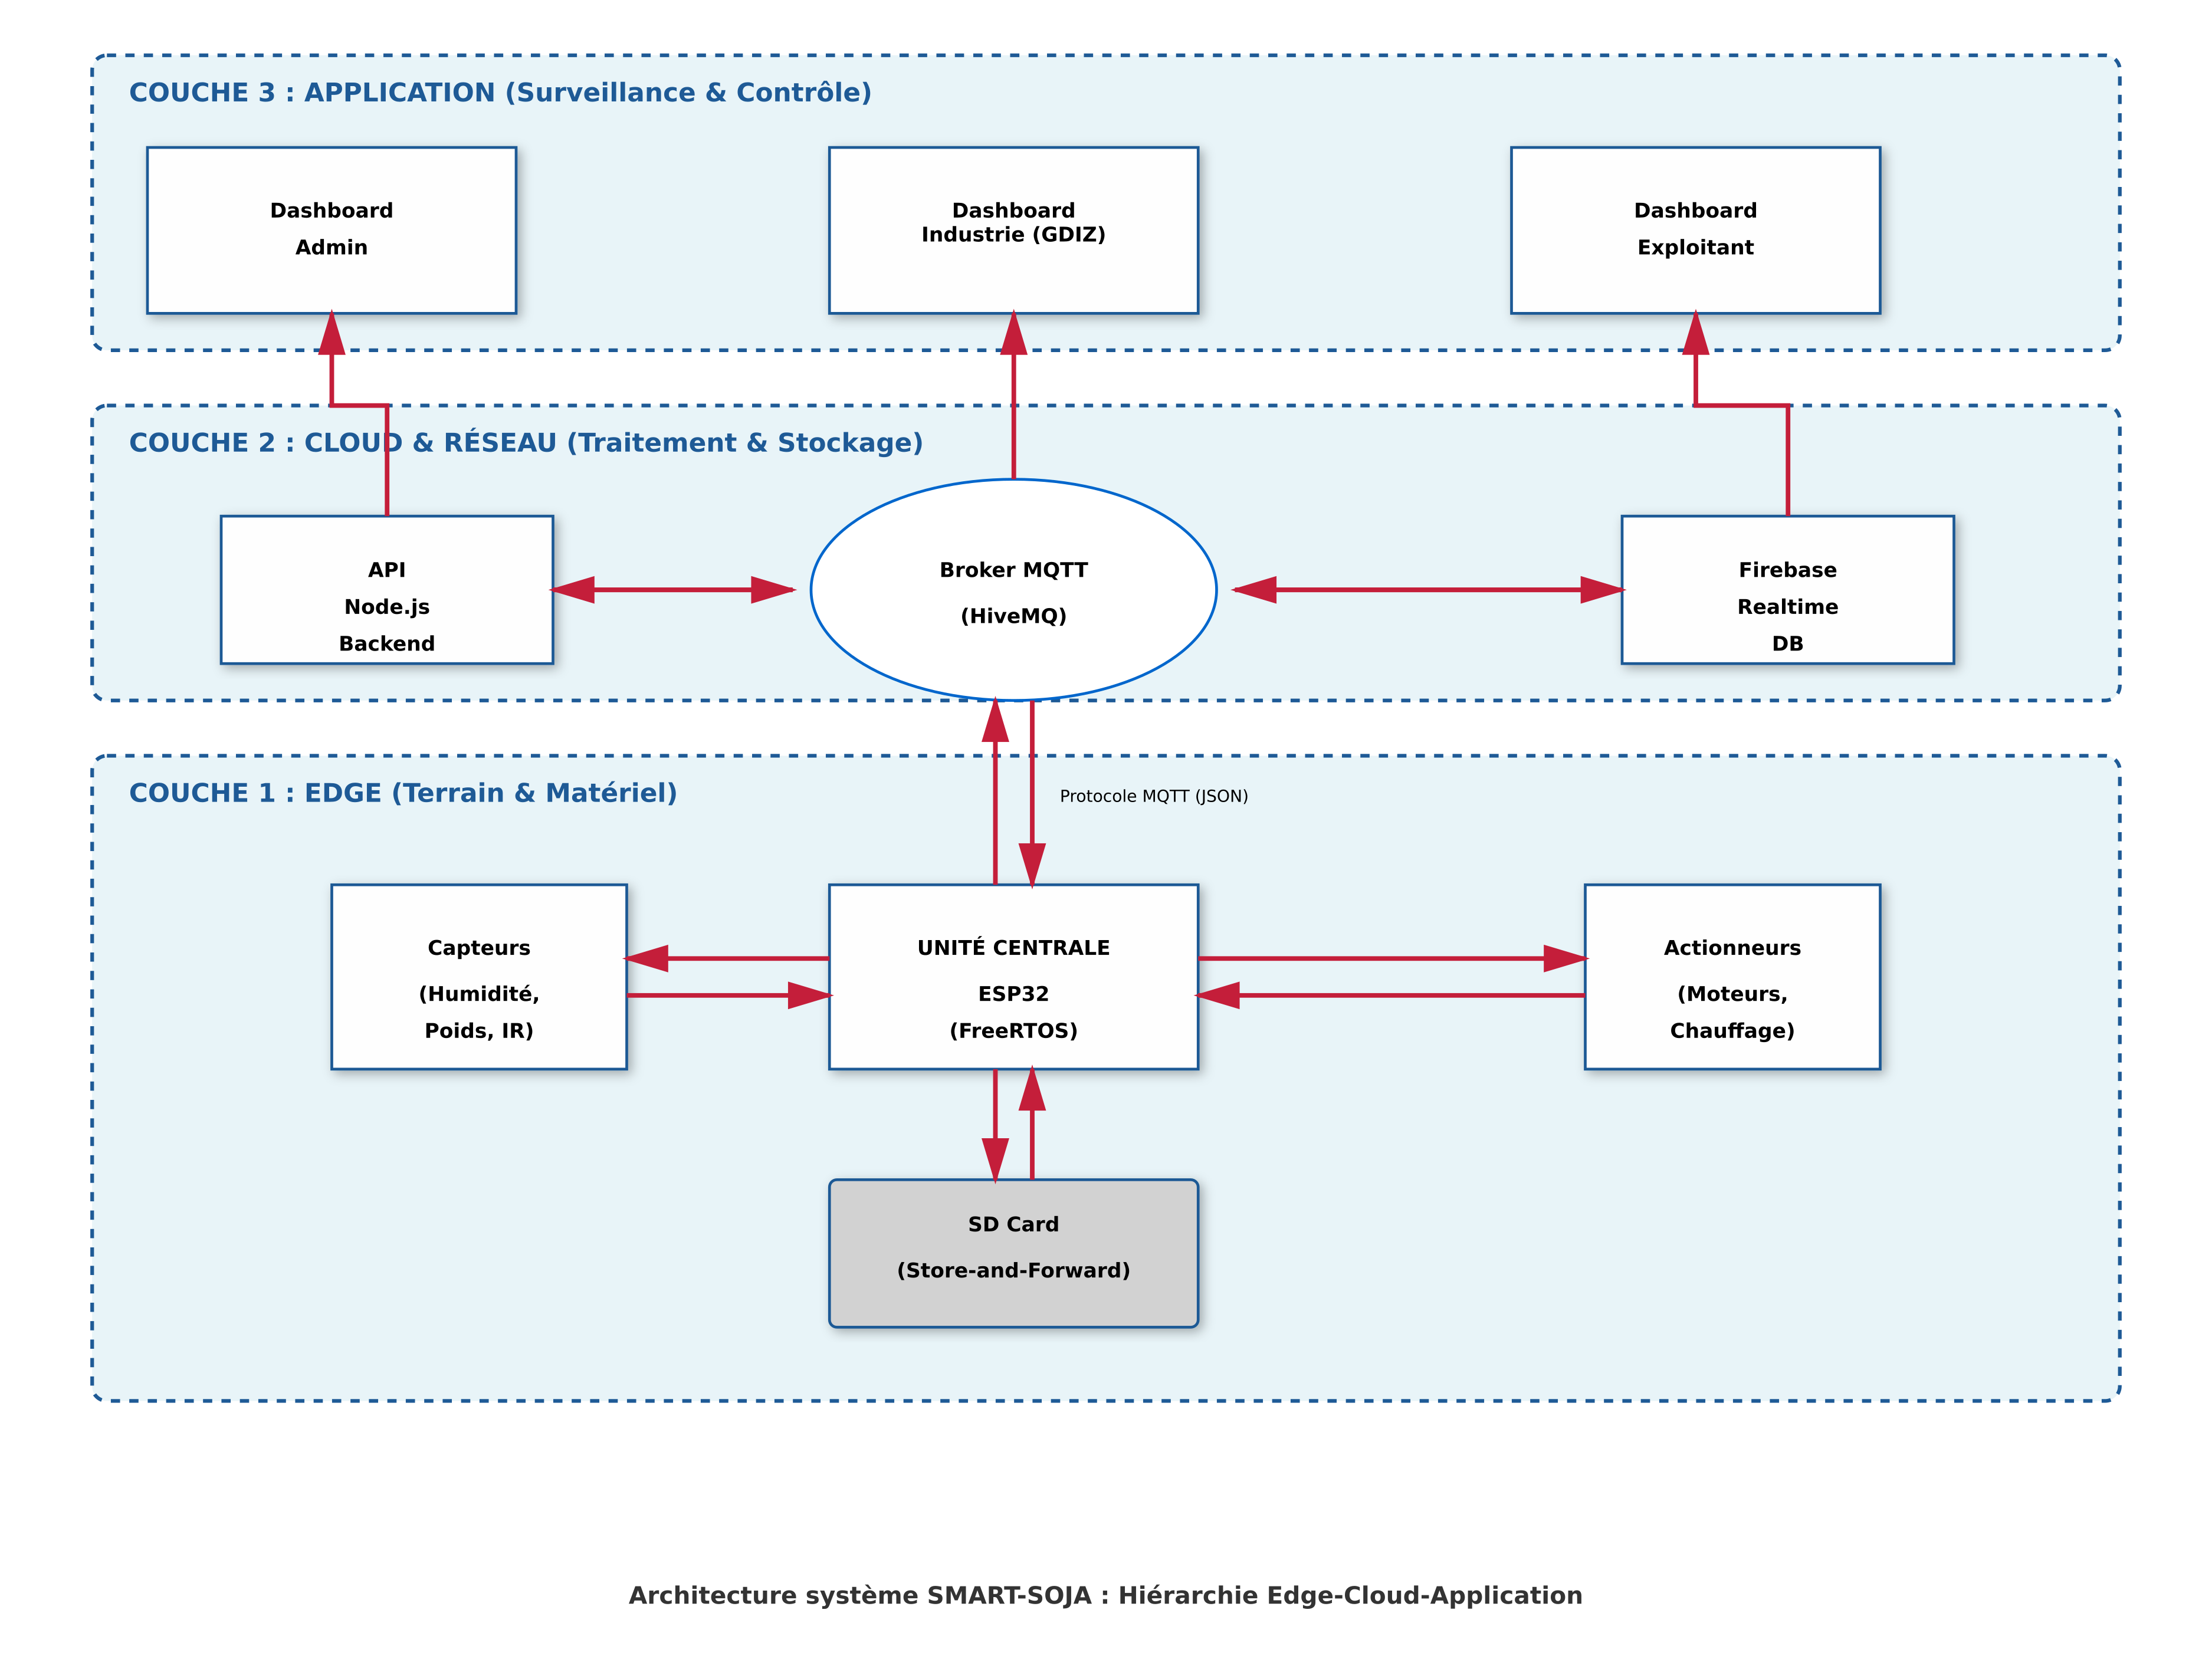
\includegraphics[width=\textwidth]{images/architecture_smart_soja.png}
    \caption{Architecture système SMART-SOJA : Hiérarchie Edge-Cloud-Application}
    \label{fig:architecture_complete}
\end{figure}
\FloatBarrier

\begin{itemize}
    \item \textbf{Couche Edge (Terrain) :} L'ESP32 gère en temps réel l'acquisition des capteurs, le pilotage des actionneurs et la logique de contrôle GRAFCET.
    \item \textbf{Couche Cloud :} Un broker MQTT (HiveMQ) relié à une API Node.js et une base Firebase assure le stockage et le traitement des données de traçabilité.
    \item \textbf{Couche Application :} Des tableaux de bord web (rôles Admin, Industrie, Exploitant) permettent le suivi à distance de chaque lot traité.
\end{itemize}

Cette architecture (Figure \ref{fig:architecture_complete}) garantit un fonctionnement autonome complet en mode déconnecté (\textit{Store-and-Forward} sur carte SD), tout en s'intégrant nativement dans une infrastructure Cloud de type Industrie 4.0. Elle permet une résilience face aux pannes de réseau fréquentes en milieu rural tout en assurant une visibilité globale pour les unités de transformation.

% -------------------------------------------------------
\section{Sous-système électronique et informatique}
% -------------------------------------------------------

\subsection{Unité de traitement : l'ESP32-WROOM-32}

Le microcontrôleur \textbf{ESP32-WROOM-32} (Figure \ref{fig:esp32_presentation}) constitue le cœur décisionnel du système \cite{esp32_datasheet}. Ses spécifications techniques sont résumées dans le Tableau \ref{tab:specs_esp32}.

\begin{table}[H]
    \caption{Spécifications techniques du microcontrôleur ESP32-WROOM-32}
    \label{tab:specs_esp32}
    \centering
    \small
    \renewcommand{\arraystretch}{1.4}
    \rowcolors{2}{white}{lightGray}
    \begin{tabularx}{\textwidth}{|L|>{\bfseries}L|}
        \hline
        \rowcolor{lightGray}
        \textbf{Caractéristique} & \textbf{Spécification} \\ \hline
        Microcontrôleur & Tensilica LX6 double cœur 240 MHz \\ \hline
        Alimentation & 5~V DC (microUSB) / 3,3~V DC (E/S) \\ \hline
        Consommation veille & 5~\textmu A (Ultra-low power) \\ \hline
        Mémoire & 520 Ko SRAM / 4 Mo Flash \\ \hline
        Connectivité & Wi-Fi 802.11 b/g/n + Bluetooth 4.2 \\ \hline
        GPIO & 30 broches (3x UART, 2x I2C, 3x SPI, 12x ADC, 2x DAC) \\ \hline
        Dimensions & 55 × 28 × 8 mm / 11 g \\ \hline
    \end{tabularx}
\end{table}

\begin{figure}[H]
    \centering
    \begin{subfigure}[b]{0.45\textwidth}
        \centering
        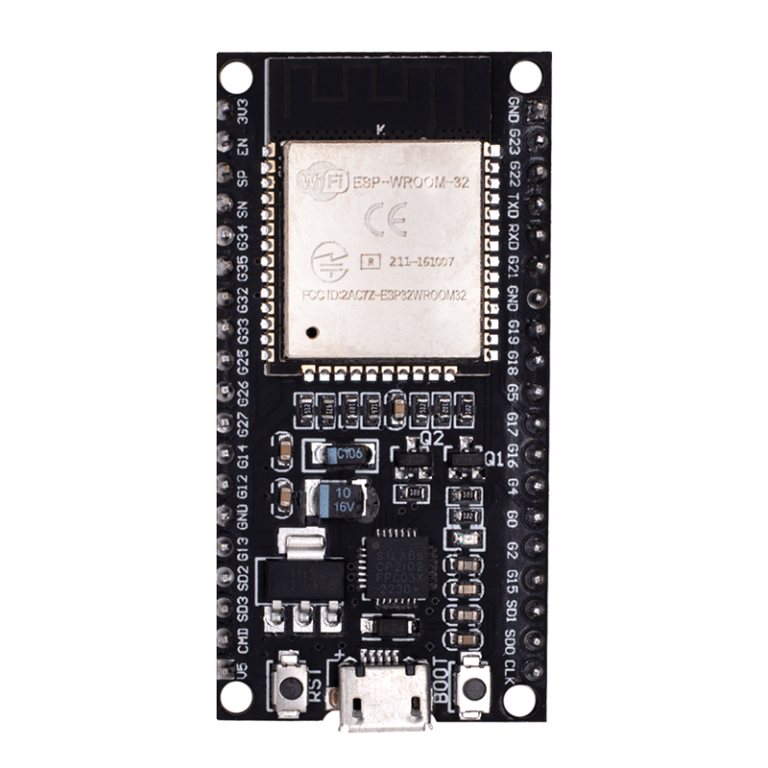
\includegraphics[width=\textwidth]{images/image_esp32.png}
        \caption{Module ESP32-WROOM-32}
    \end{subfigure}
    \hfill
    \begin{subfigure}[b]{0.45\textwidth}
        \centering
        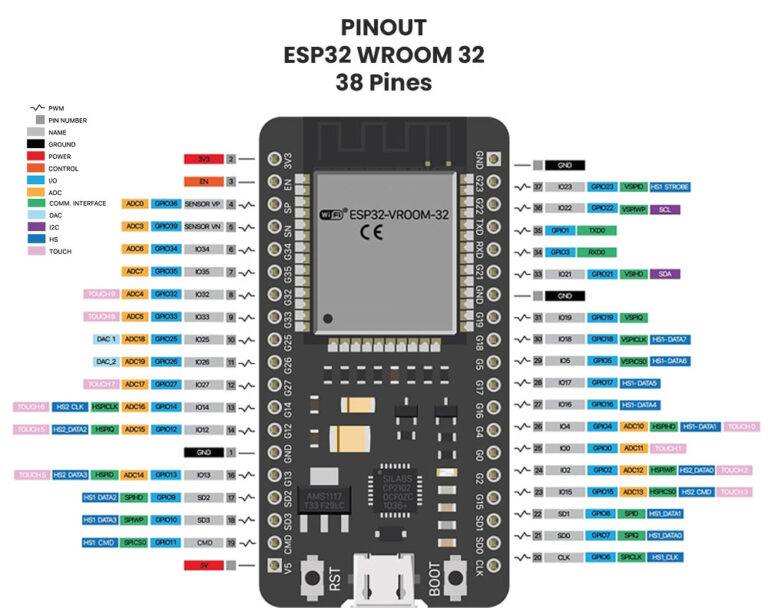
\includegraphics[width=\textwidth]{images/pinout_esp32.jpg}
        \caption{Brochage (Pinout)}
    \end{subfigure}
    \caption{Présentation du microcontrôleur ESP32}
    \label{fig:esp32_presentation}
\end{figure}
\FloatBarrier

\textbf{Justification du choix :} L'architecture Dual-Core permet de dédier un cœur au contrôle-commande temps réel (capteurs, actionneurs PWM) et l'autre à la communication Internet des objets (MQTT/WiFi), garantissant un déterminisme critique. La consommation de 5~\textmu A en veille optimise l'autonomie solaire, et les 30 GPIO offrent la flexibilité nécessaire pour tous les bus I2C, SPI et interfaces ADC du système.

\subsection{Chaîne d'acquisition : les capteurs}

Quatre capteurs stratégiques (Figure \ref{fig:capteurs_systeme}) assurent le suivi de la qualité et le déclenchement automatique des actions du GRAFCET (Tableau \ref{tab:specs_capteurs}).

\begin{table}[H]
    \caption{Spécifications détaillées de la chaîne d'acquisition}
    \label{tab:specs_capteurs}
    \centering
    \small
    \renewcommand{\arraystretch}{1.5}
    \rowcolors{2}{white}{lightGray}
    \begin{tabularx}{\textwidth}{|L|C|C|L|L|}
        \hline
        \rowcolor{lightGray}
        \textbf{Capteur} & \textbf{Plage / Précision} & \textbf{Calibration} & \textbf{Rôle} & \textbf{Limites} \\ \hline
        DHT22 & 0-100\% RH / ±2\% & Usine (1-Wire) & Humidité/Temp. ambiante & Temps réponse 2s \\ \hline
        Sonde Capacitive & 0-100\% (HR equiv.) / ±5\% & In-situ (soja sec/humide) & Humidité grains (Soil1, Soil2) & Dérive thermique \\ \hline
        IR Réflectif & 2-30 cm / Binaire & Trimpot manuel & Présence trémie/sac & Lumière ambiante \\ \hline
        Cellule de charge & 0-10 kg / ±0,1\% & Poids étalon (HX711) & Pesée finale du lot & Vibrations mécaniques \\ \hline
    \end{tabularx}
\end{table}

\begin{figure}[H]
    \centering
    \begin{subfigure}[b]{0.22\textwidth}
        \centering
        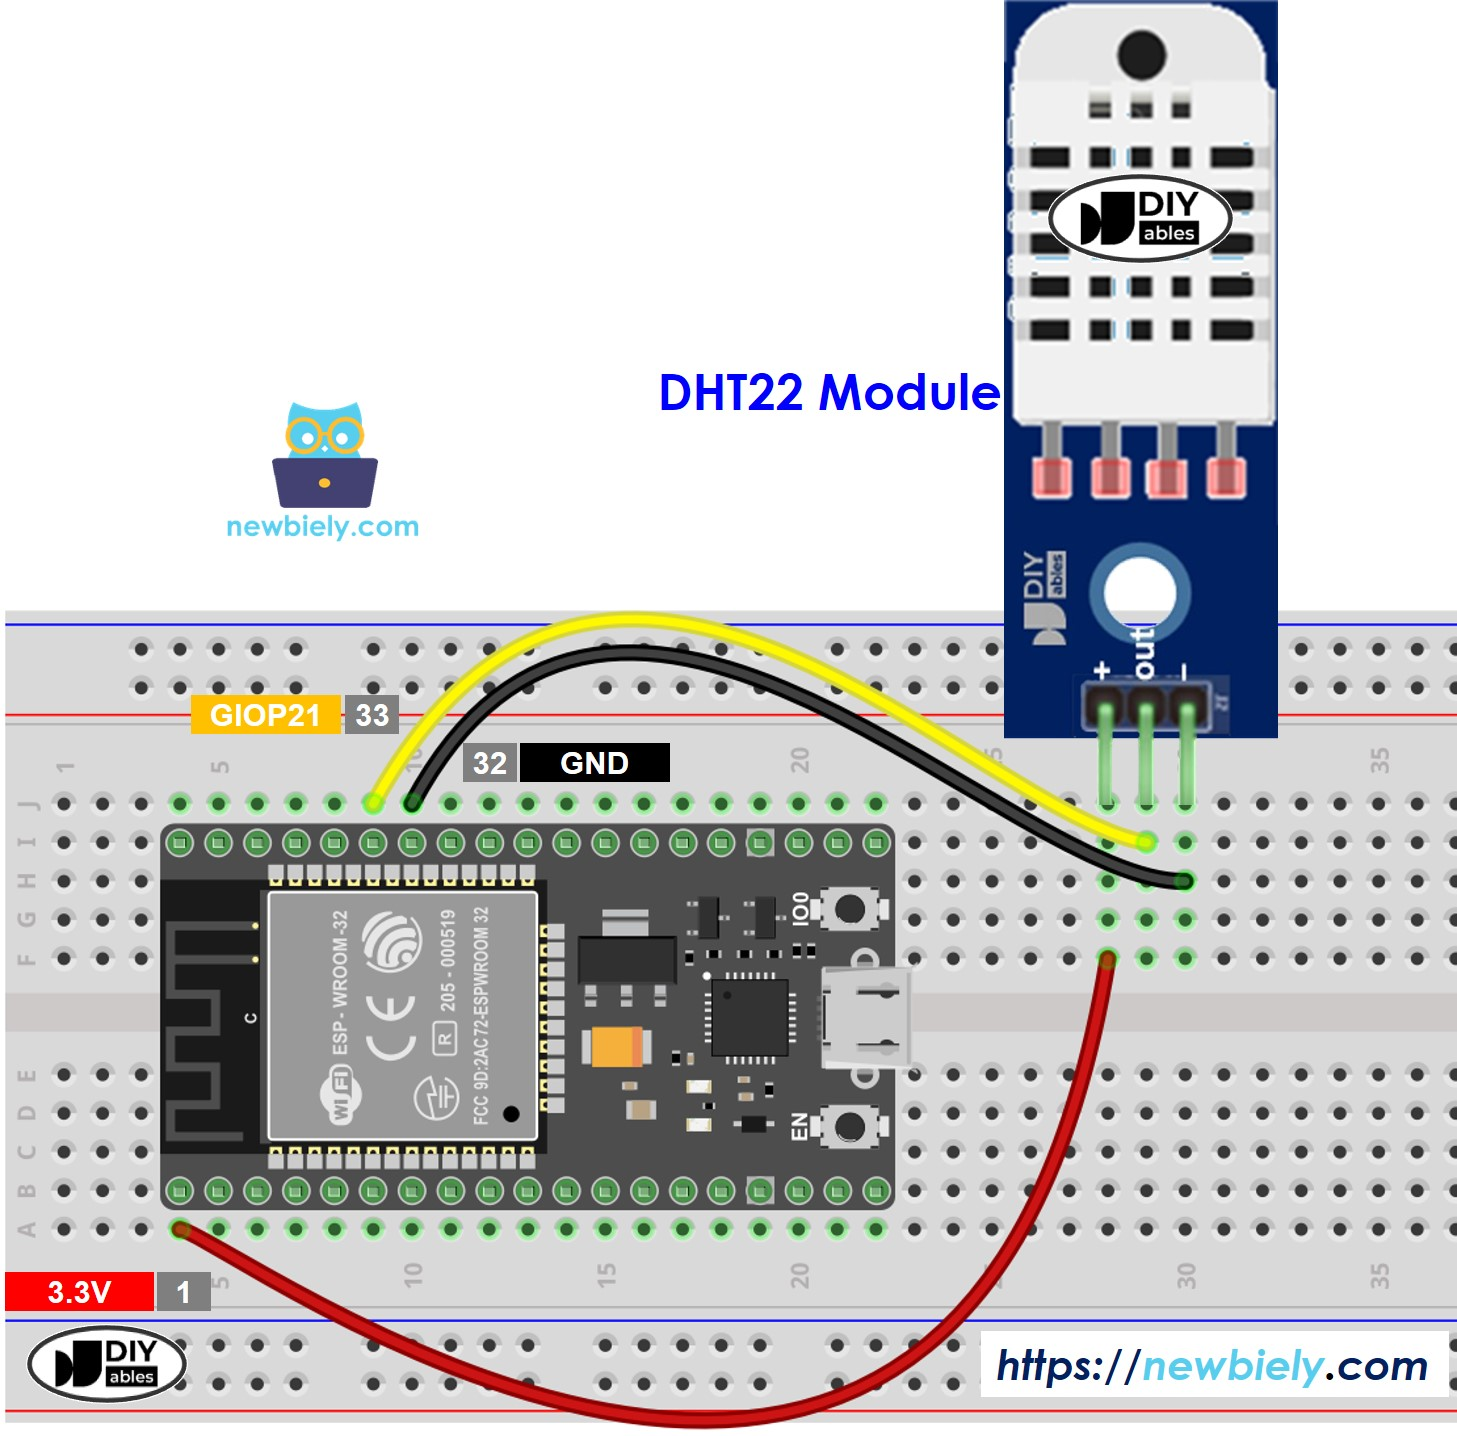
\includegraphics[width=\textwidth]{images/esp32-dht22-module-broche3.jpg}
        \caption{DHT22}
    \end{subfigure}
    \hfill
    \begin{subfigure}[b]{0.22\textwidth}
        \centering
        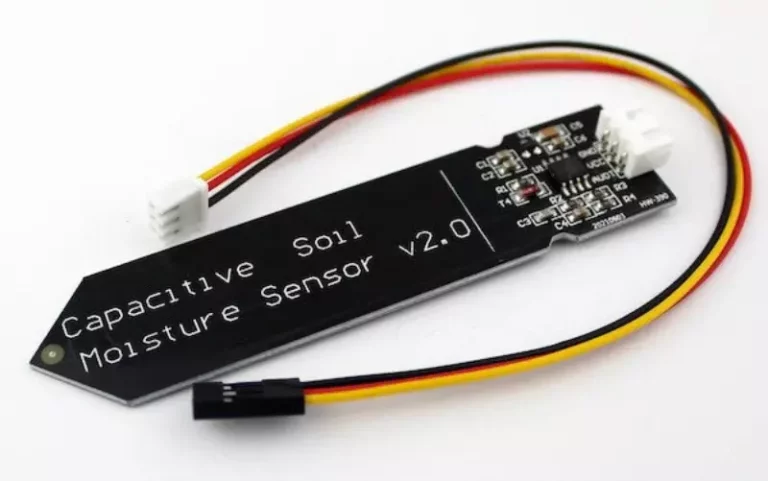
\includegraphics[width=\textwidth]{images/Capacitive-Soil-Moisture-Sensor-768x481.png}
        \caption{Sonde capacitive}
    \end{subfigure}
    \hfill
    \begin{subfigure}[b]{0.22\textwidth}
        \centering
        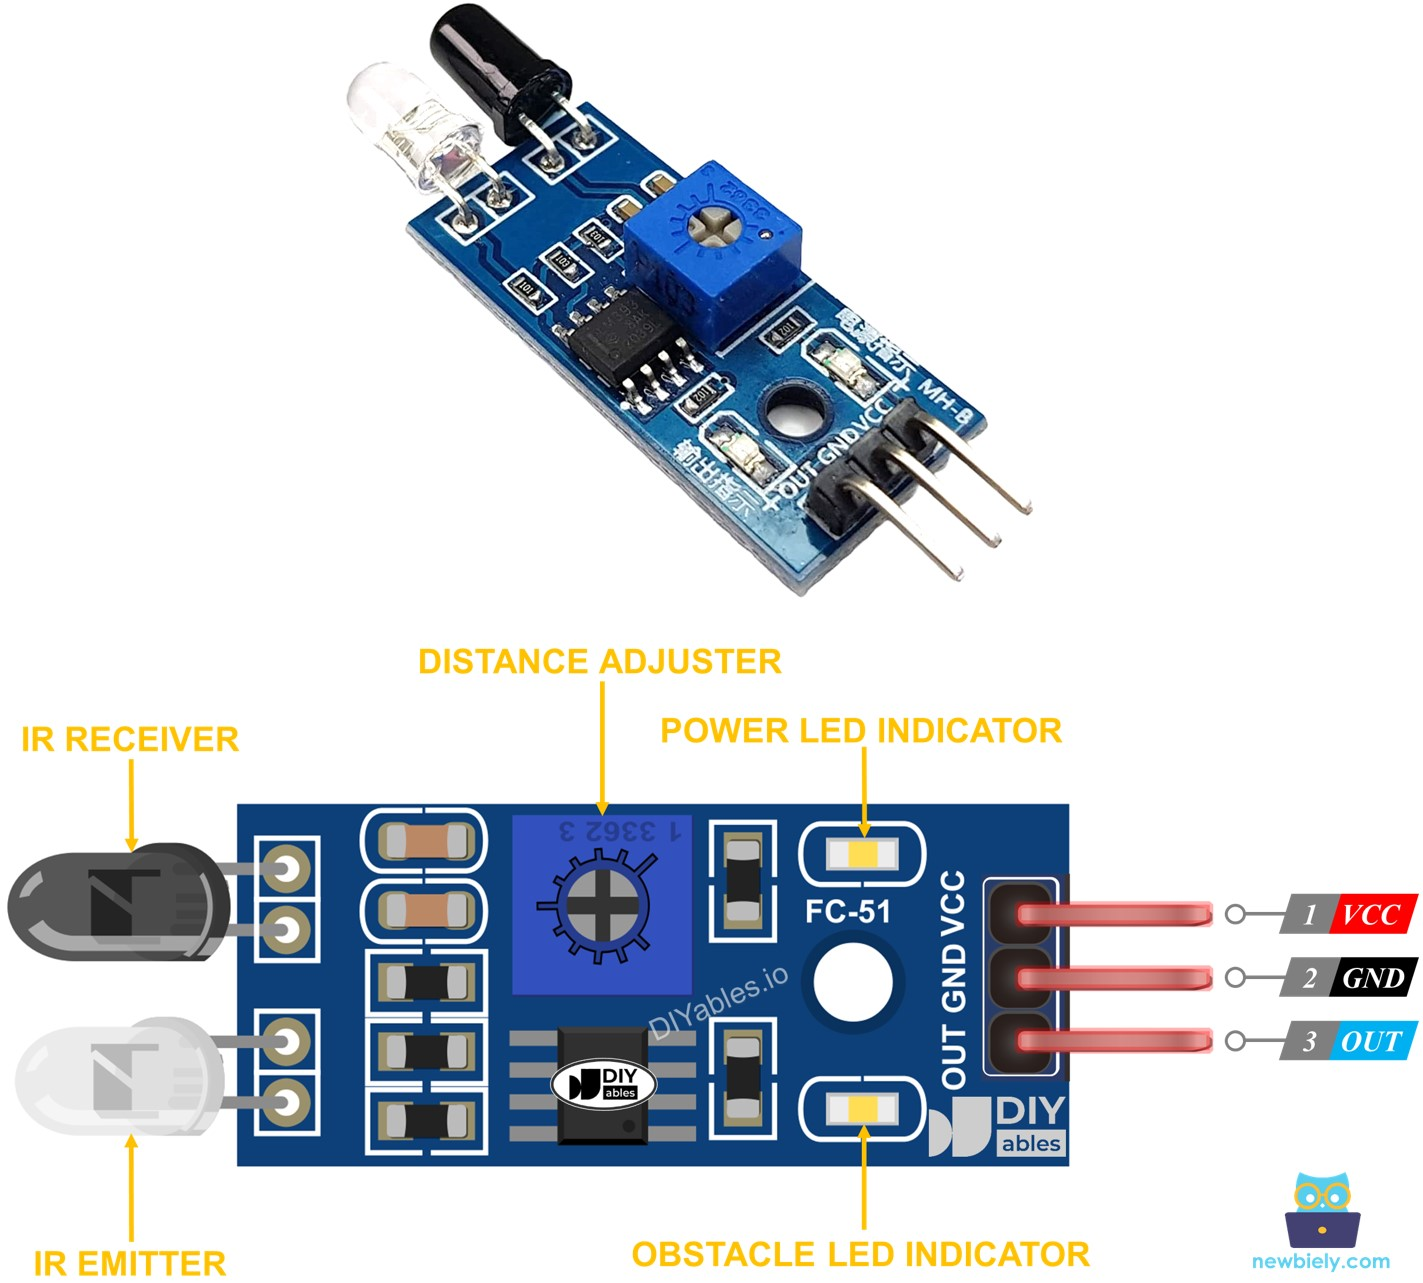
\includegraphics[width=\textwidth]{images/IR-avoidance-sensor-pinout.jpg}
        \caption{Capteur IR}
    \end{subfigure}
    \hfill
    \begin{subfigure}[b]{0.22\textwidth}
        \centering
        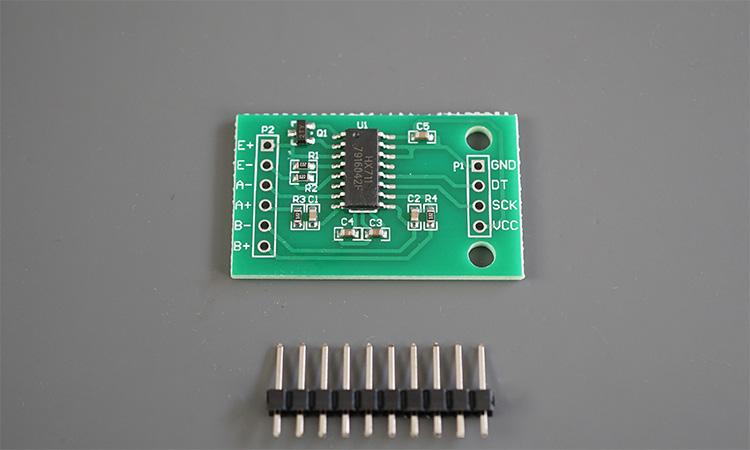
\includegraphics[width=\textwidth]{images/hx711-amplifier.jpg}
        \caption{Module HX711}
    \end{subfigure}
    \caption{Capteurs intégrés au système SMART-SOJA}
    \label{fig:capteurs_systeme}
\end{figure}
L'intégration de cette chaîne d'acquisition (Figure \ref{fig:capteurs_systeme}) permet de couvrir l'intégralité des besoins de suivi : l'humidité ambiante influe sur la cinétique de séchage, les sondes capacitives valident la qualité intrinsèque, l'infrarouge gère l'automatisation du flux et la cellule de charge certifie le poids final.

La \textbf{sonde d'humidité capacitive} mérite une attention particulière : elle mesure la constante diélectrique du milieu (eau $\approx$ 80 vs. grain sec $\approx$ 3--5), ce qui la rend insensible à la corrosion — avantage décisif pour un usage en contact direct avec les grains de soja. Deux sondes (Soil1 et Soil2) sont positionnées respectivement en haut et en bas de la zone de séchage, permettant un calcul d'humidité moyenne en deux points.

\textbf{Calibration in-situ :} La sonde capacitive délivre une tension analogique lue par le convertisseur ADC 12 bits de l'ESP32 (plage 0--4095). Une calibration en deux points est réalisée avant chaque campagne d'essai :
\begin{enumerate}
    \item \textbf{Point sec} ($H \approx 8~\%$) : un échantillon de soja séché à l'étuve est placé autour de la sonde ; la valeur ADC correspondante est enregistrée comme borne haute (soja conforme).
    \item \textbf{Point humide} ($H \approx 20~\%$) : un échantillon saturé en humidité sert de borne basse (soja non conforme).
\end{enumerate}
Une interpolation linéaire entre ces deux bornes permet de convertir toute lecture ADC intermédiaire en un taux d'humidité exprimé en pourcentage. Cette méthode simple mais robuste est validée par comparaison avec les mesures de l'hygromètre de référence Testo 608-H2, avec un écart maximal observé de $\pm 5~\%$ conformément à la spécification du capteur (Tableau~\ref{tab:specs_capteurs}).

\subsection{Chaîne d'action : actionneurs et interface de puissance}

Le pilotage des charges électromécaniques (12~V, forts courants) depuis un microcontrôleur 3,3~V nécessite des interfaces de puissance adaptées (Figure \ref{fig:actionneurs_systeme}). Le Tableau \ref{tab:specs_actionneurs} récapitule les actionneurs du système.

\begin{table}[H]
    \caption{Spécifications détaillées de la chaîne d'action}
    \label{tab:specs_actionneurs}
    \centering
    \small
    \renewcommand{\arraystretch}{1.5}
    \rowcolors{2}{white}{lightGray}
    \begin{tabularx}{\textwidth}{|L|C|L|L|}
        \hline
        \rowcolor{lightGray}
        \textbf{Actionneur} & \textbf{Puissance / Courant} & \textbf{Critère de dimensionnement} & \textbf{Protections} \\ \hline
        Moteurs JGA25 & 3~W / 0,5~A (max 1,2~A) & Couple de rotation pour tamis et vis & Diode roue libre \\ \hline
        MOSFET IRLZ44N & 175~W / 47~A (max) & Compatibilité \textit{Logic Level} (3,3~V) & Résistance de Gate \\ \hline
        Servo SG90 & 1,5~W / 0,1~A à 0,5~A & Couple de 1,3 kg.cm pour la vanne & Condensateur de filtrage \\ \hline
        Résistance & 12~W / 1~A & Delta Température pour séchage & Fusible thermique \\ \hline
        Ventilateur DC & 1,8~W / 0,15~A & Flux d'air de 15 CFM pour extraction & Diode roue libre \\ \hline
    \end{tabularx}
\end{table}

\begin{figure}[H]
    \centering
    \begin{subfigure}[b]{0.19\textwidth}
        \centering
        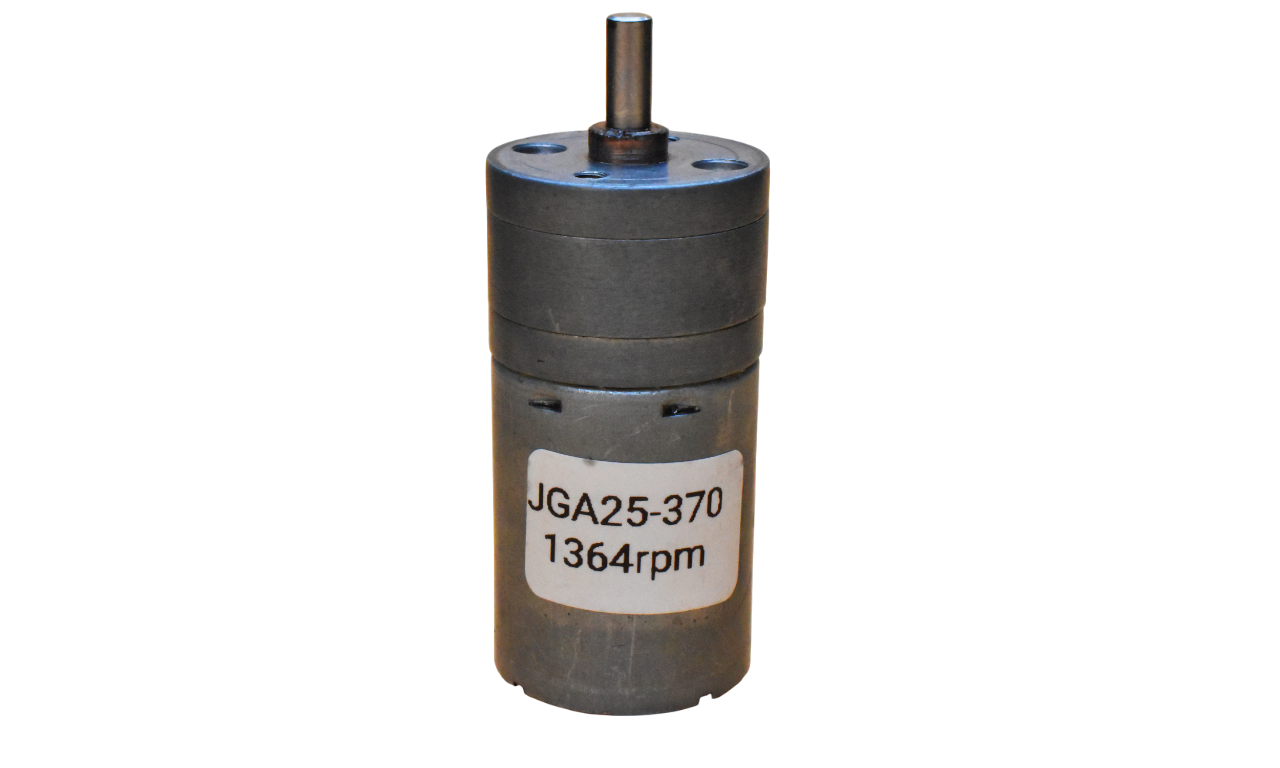
\includegraphics[width=\textwidth]{images/moteur_jga25-370 1364.png}
        \caption{Moteur JGA25}
    \end{subfigure}
    \hfill
    \begin{subfigure}[b]{0.19\textwidth}
        \centering
        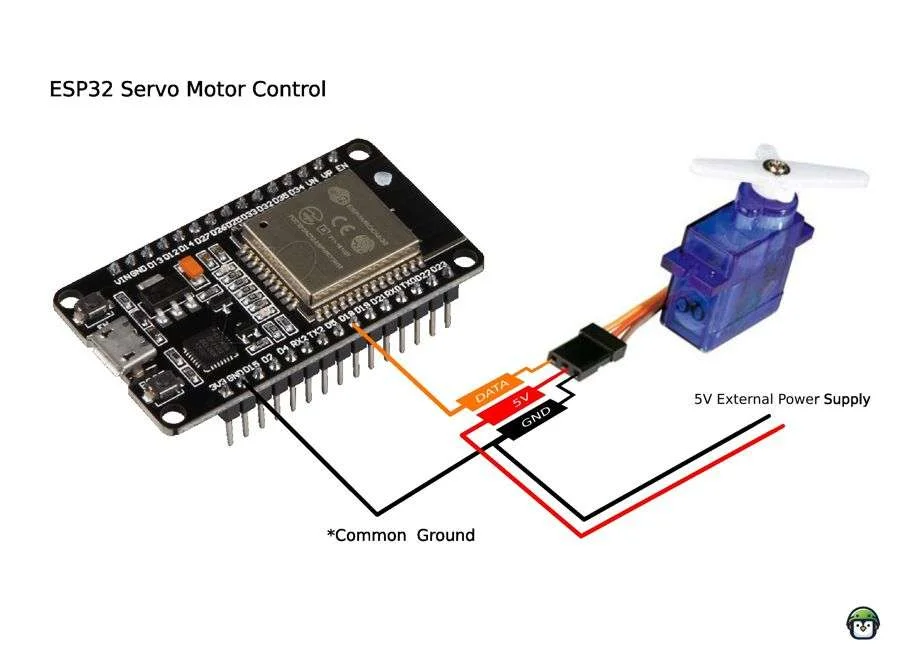
\includegraphics[width=\textwidth]{images/samgalope.dev-devdigest-ESP32-SERVO-SG90.png}
        \caption{Servo SG90}
    \end{subfigure}
    \hfill
    \begin{subfigure}[b]{0.19\textwidth}
        \centering
        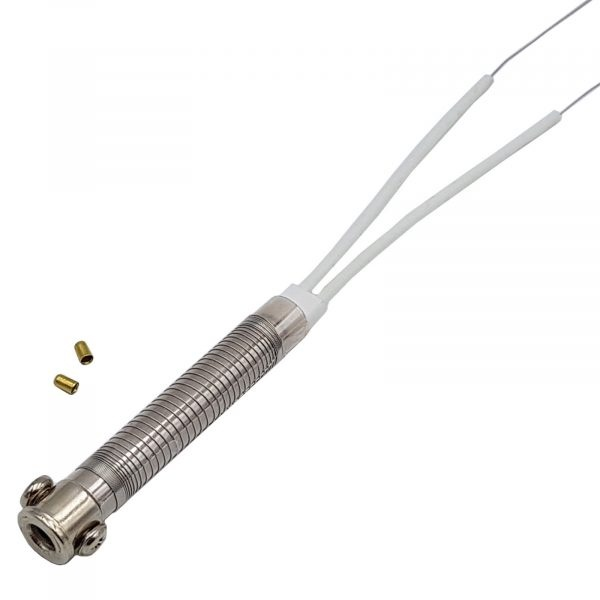
\includegraphics[width=\textwidth]{images/resistance_chauffante.jpg}
        \caption{Résistance}
    \end{subfigure}
    \hfill
    \begin{subfigure}[b]{0.19\textwidth}
        \centering
        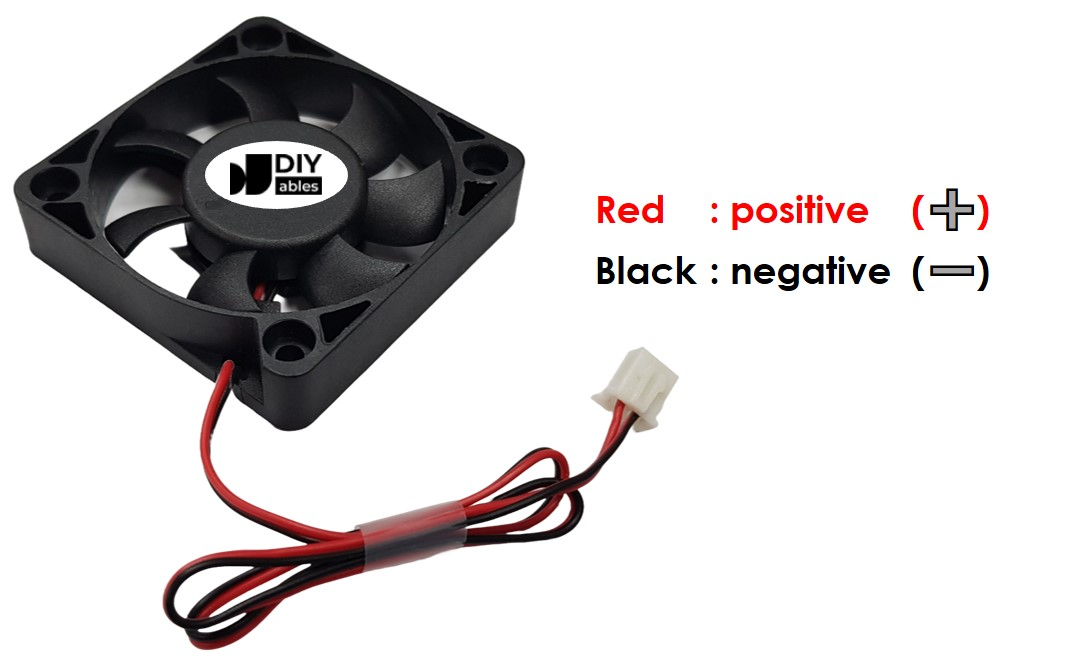
\includegraphics[width=\textwidth]{images/fan-pinout.jpg}
        \caption{Ventilateur}
    \end{subfigure}
    \hfill
    \begin{subfigure}[b]{0.19\textwidth}
        \centering
        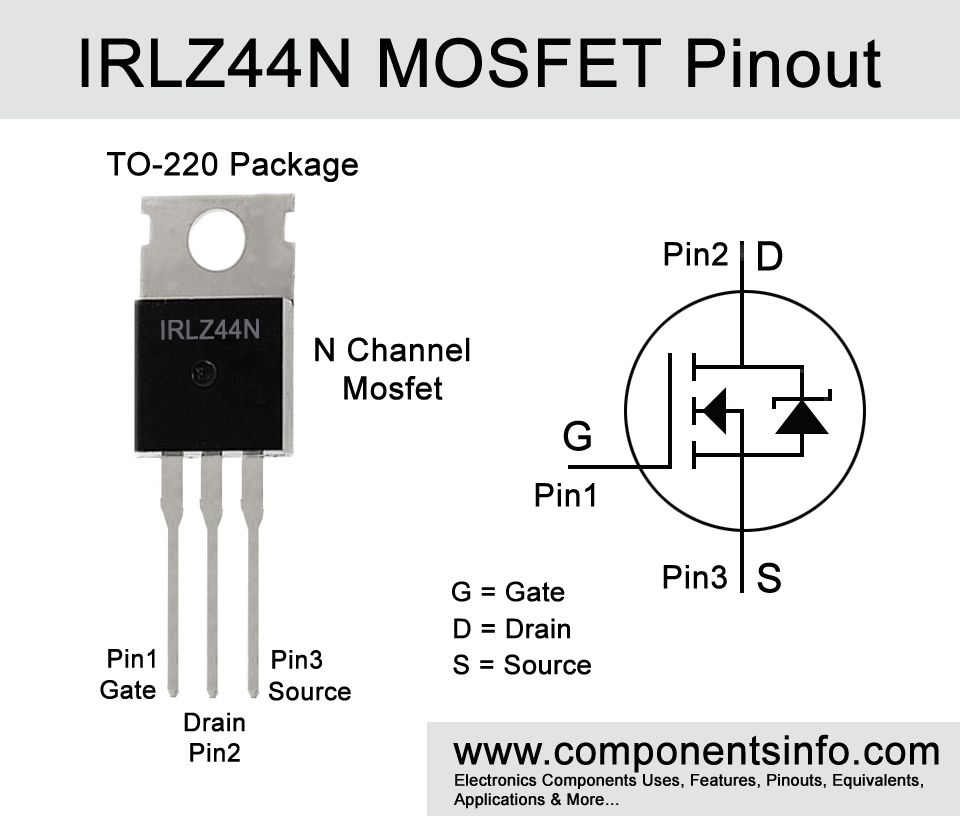
\includegraphics[width=\textwidth]{images/irlz44n-pinout-equivalent.png}
        \caption{MOSFET}
    \end{subfigure}
    \caption{Actionneurs et interface de puissance du système}
    \label{fig:actionneurs_systeme}
\end{figure}
\FloatBarrier

Le \textbf{MOSFET IRLZ44N} est retenu car, contrairement aux MOSFET standards nécessitant 10~V de commande, ce modèle \textit{Logic Level} se sature directement avec les 3,3~V de l'ESP32. Il peut commuter jusqu'à 47~A avec une résistance interne de seulement 0,022~$\Omega$, permettant un pilotage PWM précis des moteurs et de la résistance chauffante sans échauffement excessif \cite{irlz44n_datasheet}. Il convient de noter que la valeur de 175~W indiquée dans le Tableau~\ref{tab:specs_actionneurs} correspond à la puissance maximale absolue que ce composant est physiquement capable de dissiper (selon sa fiche technique, sous conditions de refroidissement optimal), et non à la puissance effectivement consommée par le prototype SMART-SOJA dont le bilan total s'élève à 37,85~W (Tableau~\ref{tab:specs_energie}).

\subsection{Interfaces homme-machine et traçabilité locale}

\begin{table}[H]
    \caption{Interfaces locales et modules de traçabilité}
    \label{tab:specs_ihm}
    \centering
    \small
    \renewcommand{\arraystretch}{1.6}
    \rowcolors{2}{white}{lightGray}
    \begin{tabularx}{\textwidth}{|L|>{\bfseries}C|L|}
        \hline
        \rowcolor{lightGray}
        \textbf{Périphérique} & \textbf{Protocole} & \textbf{Rôle fonctionnel} \\ \hline
        LCD 16×2 & I2C & Affichage en temps réel des métriques et états du système. \\ \hline
        Lecteur MicroSD & SPI & Enregistrement local des données en mode \textit{Store-and-Forward}. \\ \hline
        Potentiomètres ($\times 2$) & ADC (12 bits) & Réglage manuel de la vitesse des moteurs par l'opérateur. \\ \hline
        Boutons ON/OFF & GPIO Pull-Up & Démarrage et arrêt sécurisé du cycle de traitement. \\ \hline
        LEDs \& Buzzer & Digital/PWM & Signalisation d'état (mode, alerte, erreur). \\ \hline
    \end{tabularx}
\end{table}

Le système intègre également des interfaces de dialogue local (Figure \ref{fig:ihm_systeme}) pour l'opérateur de terrain.

\begin{figure}[H]
    \centering
    \begin{subfigure}[b]{0.19\textwidth}
        \centering
        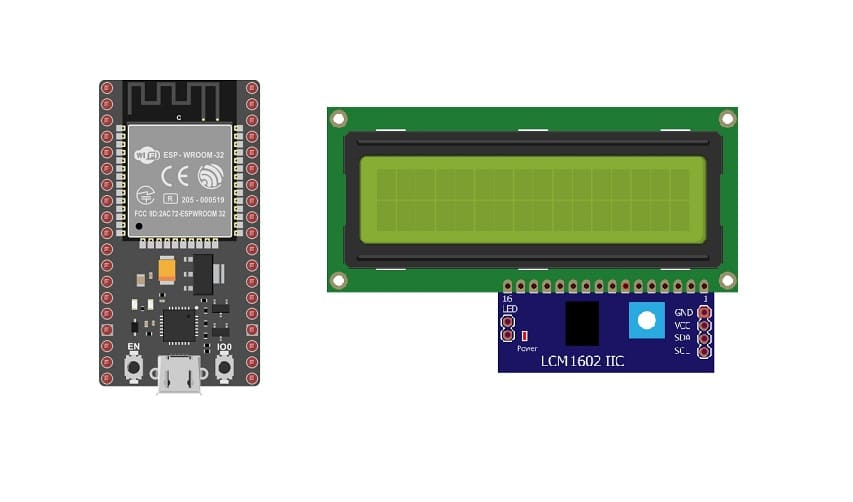
\includegraphics[width=\textwidth]{images/esp32-lcd-i2c-single.jpg}
        \caption{LCD 16x2}
    \end{subfigure}
    \hfill
    \begin{subfigure}[b]{0.19\textwidth}
        \centering
        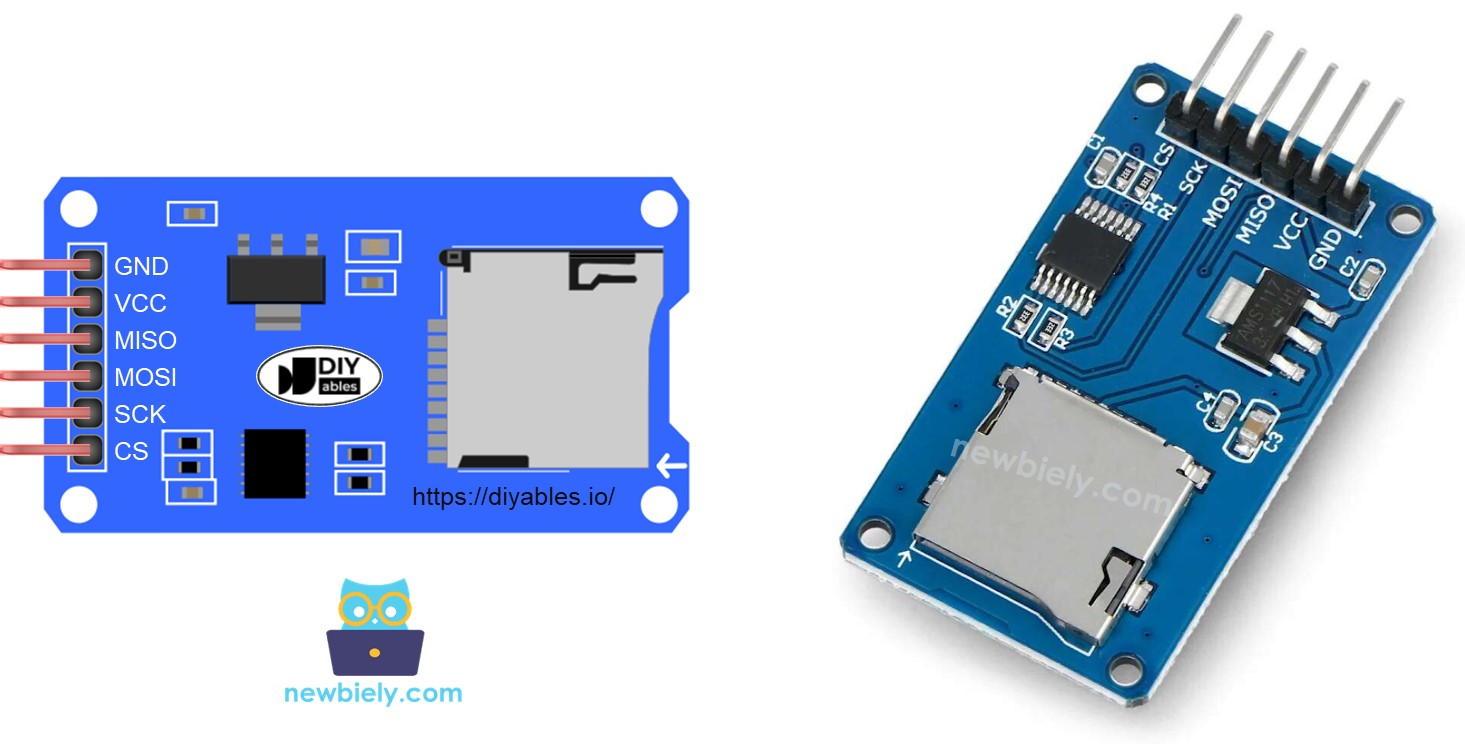
\includegraphics[width=\textwidth]{images/micro-sd-card-module-pinout.jpg}
        \caption{Lecteur SD}
    \end{subfigure}
    \hfill
    \begin{subfigure}[b]{0.19\textwidth}
        \centering
        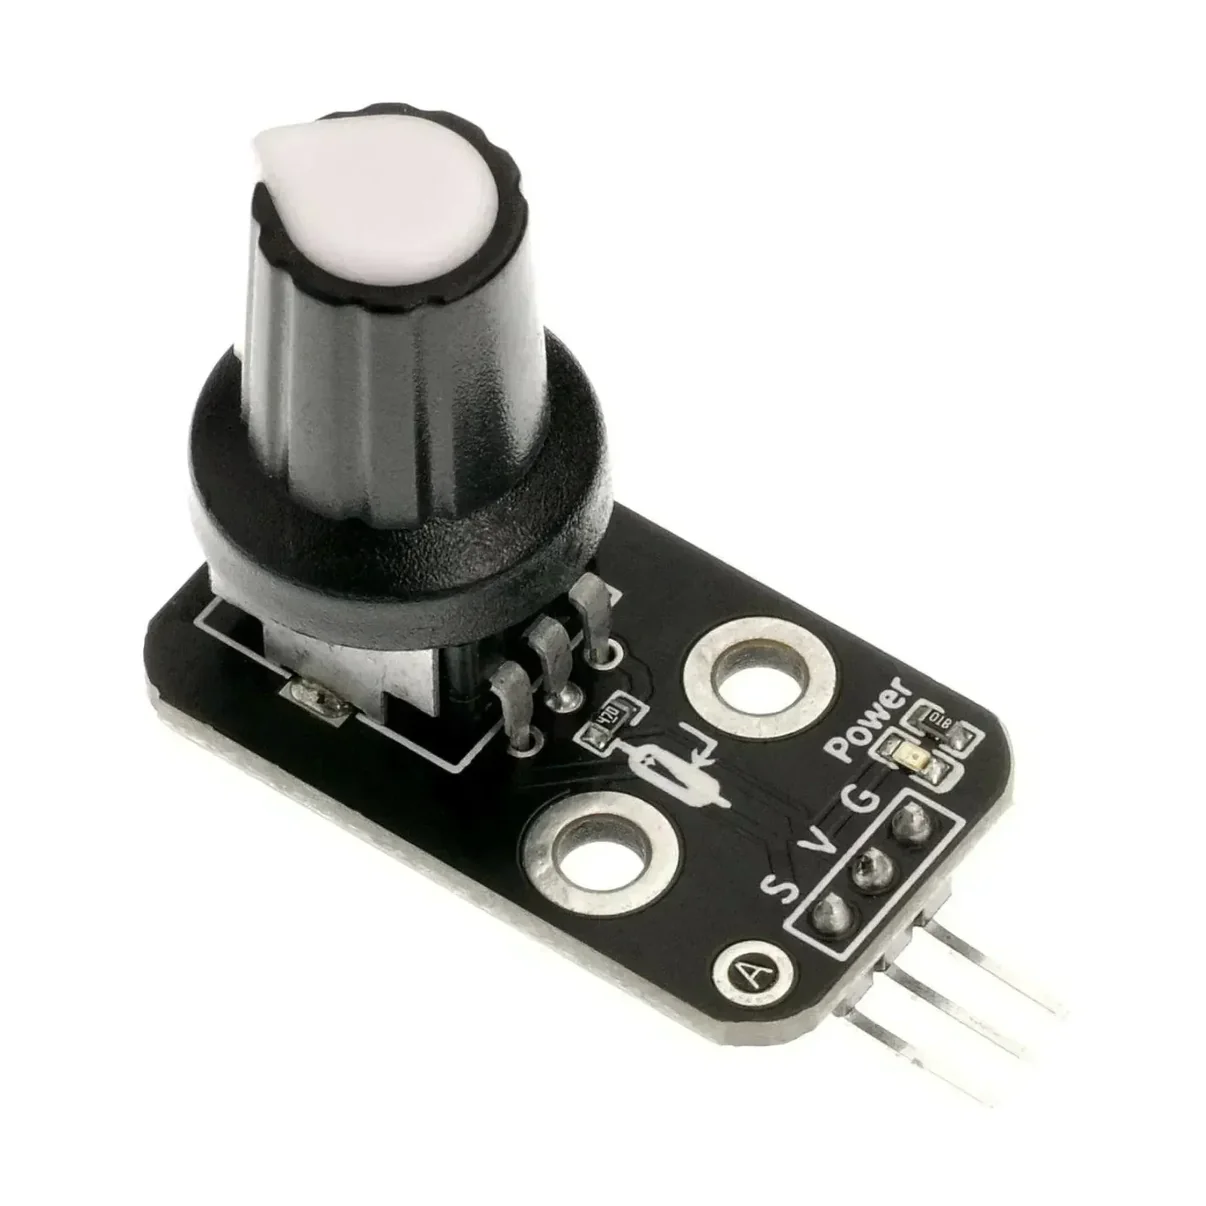
\includegraphics[width=\textwidth]{images/potentiometre_rotatif.png}
        \caption{Potentiomètre}
    \end{subfigure}
    \hfill
    \begin{subfigure}[b]{0.19\textwidth}
        \centering
        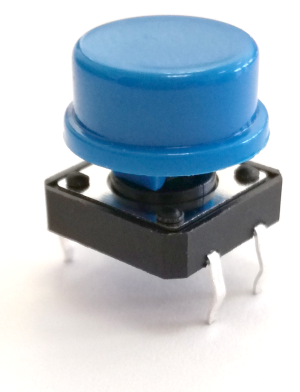
\includegraphics[width=\textwidth]{images/bouton_bleu.png}
        \caption{Boutons}
    \end{subfigure}
    \hfill
    \begin{subfigure}[b]{0.19\textwidth}
        \centering
        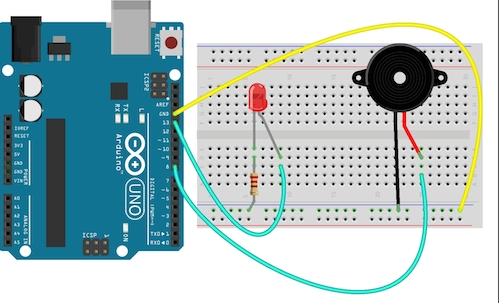
\includegraphics[width=\textwidth]{images/buzzer + led.jpg}
        \caption{Signalisation}
    \end{subfigure}
    \caption{Interfaces locales et modules de traçabilité}
    \label{fig:ihm_systeme}
\end{figure}
\FloatBarrier

Le \textbf{lecteur MicroSD} (interface SPI, format FAT32) joue un rôle critique pour la traçabilité : en l'absence de réseau WiFi, toutes les métriques de traitement sont sauvegardées localement et retransmises automatiquement au broker MQTT dès la reconnexion — mécanisme dit de \textit{Store-and-Forward}.

% -------------------------------------------------------
\section{Sous-système énergétique : autonomie solaire}
% -------------------------------------------------------
Pour garantir un fonctionnement ininterrompu en milieu rural hors réseau, le système \textbf{SMART-SOJA} repose sur une alimentation photovoltaïque dimensionnée selon les principes de calcul de capacité batterie pour systèmes isolés \cite{labouret2017}. Le bilan de puissance des actionneurs est détaillé dans le Tableau \ref{tab:specs_energie} et le synoptique complet de la chaîne de puissance est présenté en \textbf{Annexe \ref{annexe:schema_alim}}.

\begin{table}[H]
    \caption{Bilan énergétique et spécifications d'alimentation}
    \label{tab:specs_energie}
    \centering
    \small
    \renewcommand{\arraystretch}{1.5}
    \rowcolors{2}{white}{lightGray}
    \begin{tabularx}{\textwidth}{|L|L|}
        \hline
        \rowcolor{lightGray}
        \textbf{Paramètre Énergétique} & \textbf{Valeur / Spécification} \\ \hline
        Production (Panneau) & Monocristallin 50~W (Peak) \\ \hline
        Stockage (Batterie) & Plomb-acide 12~V 20~Ah (240~Wh) \\ \hline
        Bilan de puissance crête & 37,85~W (Toutes charges ON) \\ \hline
        Consommation journalière est. & environ 113,5~Wh (pour 3h de travail) \\ \hline
        Autonomie théorique (sans soleil) & environ 1 jour (à 50\% de décharge) \\ \hline
        Conversion & Régulateurs Buck LM2596 (Efficacité > 85\%) \\ \hline
    \end{tabularx}
\end{table}

\textbf{Dimensionnement du système :} Pour valider les choix technologiques du kit de l'entreprise \textbf{QOTTO} (Batterie de 20~Ah et panneau de 50~W), nous avons procédé à un dimensionnement basé sur le besoin réel du prototype.

\begin{enumerate}
    \item \textbf{Étape 1 — Bilan de puissance crête :} La puissance totale est la somme des consommations réelles des composants du prototype (incluant deux résistances et deux ventilateurs pour le séchage) :
    \[ P_{tot} = \underbrace{9,0\text{W}}_{\text{2 Moteurs}} + \underbrace{\mathbf{24,0\text{W}}}_{\text{2 Résistances}} + \underbrace{\mathbf{3,6\text{W}}}_{\text{2 Ventilos}} + \underbrace{1,25\text{W}}_{\text{ESP32}} = \mathbf{37,85~\text{W}} \]
    
    \item \textbf{Étape 2 — Énergie consommée par jour ($E_j$) :} En considérant une utilisation du prototype pendant \textbf{3 heures par jour} (soit environ 18 cycles de traitement), l'énergie totale consommée est :
    \[ E_{jour} = 37,85~\text{W} \times 3~\text{h} \approx \mathbf{113,5~\text{Wh/jour}} \]
    
    \item \textbf{Étape 3 — Validation de la batterie :} La batterie de 12~V et 20~Ah possède une capacité totale de \textbf{240~Wh}. En limitant la décharge à 50~\% pour prolonger sa durée de vie (standard pour les batteries au plomb), l'énergie réellement disponible est de \textbf{120~Wh}.
    \begin{itemize}
        \item \textbf{Conclusion :} 120~Wh (disponibles) $>$ 113,5~Wh (besoin), la batterie est donc bien dimensionnée pour couvrir une session de travail quotidienne en autonomie.
    \end{itemize}

    \item \textbf{Étape 4 — Validation du panneau solaire :} Avec un ensoleillement moyen de 5 heures par jour au Bénin, le panneau de 50~W produit :
    \[ E_{produite} = 50~\text{W} \times 5~\text{h} = \mathbf{250~\text{Wh/jour}} \]
    \begin{itemize}
        \item \textbf{Conclusion :} 250~Wh (produits) $>$ 113,5~Wh (besoin), le panneau recharge la batterie très facilement, offrant une marge de sécurité confortable pour compenser les jours de faible ensoleillement.
    \end{itemize}
\end{enumerate}

% -------------------------------------------------------
\section{Sous-système mécanique : architecture modulaire}
% -------------------------------------------------------
La conception mécanique repose sur une structure modulaire composée d'un châssis porteur accueillant quatre blocs fonctionnels amovibles. Les matériaux ont été sélectionnés selon un compromis robustesse/coût de prototypage (Tableau \ref{tab:specs_mecanique}). Des photographies des matériaux bruts utilisés sont consultables en \textbf{Annexe \ref{annexe:materiaux_mecaniques}}.

\begin{table}[H]
    \caption{Spécifications mécaniques, contraintes et justification des matériaux}
    \label{tab:specs_mecanique}
    \centering
    \small
    \renewcommand{\arraystretch}{1.5}
    \rowcolors{2}{white}{lightGray}
    \begin{tabularx}{\textwidth}{|L|C|L|L|}
        \hline
        \rowcolor{lightGray}
        \textbf{Élément} & \textbf{Masse (kg)} & \textbf{Contrainte / Rigidité} & \textbf{Justification Matériau} \\ \hline
        Châssis porteur & 12,0 & Compression / Haute & Acier (Tubes 40~mm) : Robustesse et soudabilité \\ \hline
        Support Tamis & 0,293 & Vibration / Haute & Inox 304 : Résistance à la corrosion et hygiène \\ \hline
        Support Capteur & 0,1 & Flexion / Moyenne & PLA (3D) : Précision et légèreté \\ \hline
        Roulettes (×4) & 2,0 & Chocs / Élastique & Caoutchouc HD : Absorption des vibrations \\ \hline
    \end{tabularx}
\end{table}
\FloatBarrier

Les quatre blocs fonctionnels (alimentation, nettoyage, séchage et pesée) sont conçus pour être retirés individuellement du châssis. Ce système de glissières et connecteurs rapides facilite grandement la maintenance en milieu rural, évitant ainsi le démontage intégral de la machine.



% -------------------------------------------------------
\section{Méthodologie logicielle : contrôle temps réel}
% -------------------------------------------------------

\subsection{Le système multitâche FreeRTOS}
La gestion simultanée de la sécurité, du contrôle et de la communication Internet des objets sur l'ESP32 nécessite un ordonnancement rigoureux des tâches. Nous utilisons \textbf{FreeRTOS} \cite{freeRTOS}, un noyau temps réel miniature qui offre :
\begin{itemize}
    \item \textbf{Déterminisme :} La lecture des capteurs et le pilotage des actionneurs ne sont jamais interrompus par les tâches réseau.
    \item \textbf{Gestion Multi-Core :} Les deux cœurs de l'ESP32 sont répartis selon la criticité des tâches.
    \item \textbf{Hiérarchie des priorités :} Les tâches de sécurité préemptent systématiquement toutes les autres.
\end{itemize}

Cette organisation logicielle est détaillée dans le Tableau \ref{tab:freertos_sched}.

\begin{table}[H]
    \caption{Hiérarchie et configuration de l'ordonnanceur FreeRTOS}
    \label{tab:freertos_sched}
    \centering
    \small
    \renewcommand{\arraystretch}{1.5}
    \rowcolors{2}{white}{lightGray}
    \begin{tabularx}{\textwidth}{|L|C|L|L|}
        \hline
        \rowcolor{lightGray}
        \textbf{Tâche} & \textbf{Priorité} & \textbf{Justification} & \textbf{Risque en cas de latence} \\ \hline
        \textbf{Task\_Safety} & 4 (Max) & Sécurité critique (Arrêt, Surchauffe) & Endommagement du matériel \\ \hline
        \textbf{Task\_Control} & 3 (Haute) & Ordonnancement GRAFCET & Conflits d'états et blocages \\ \hline
        \textbf{Task\_Sensing} & 2 (Moy.) & Acquisition capteurs (Filtrage) & Mesures erronées ou bruitées \\ \hline
        \textbf{Task\_Actuators} & 2 (Moy.) & Pilotage PWM et Servomoteurs & Réactivité saccadée \\ \hline
        \textbf{Task\_LCD} & 1 (Faible) & Interface locale (I2C) & Affichage figé (non critique) \\ \hline
        \textbf{Task\_MQTT} & 1 (Faible) & Communication Internet des objets et SD & Perte de traçabilité \\ \hline
    \end{tabularx}
\end{table}

Le chronogramme de la Figure \ref{fig:freertos_chronogramme} illustre la dynamique de l'ordonnancement préemptif sur l'ESP32.

\begin{figure}[H]
    \centering
    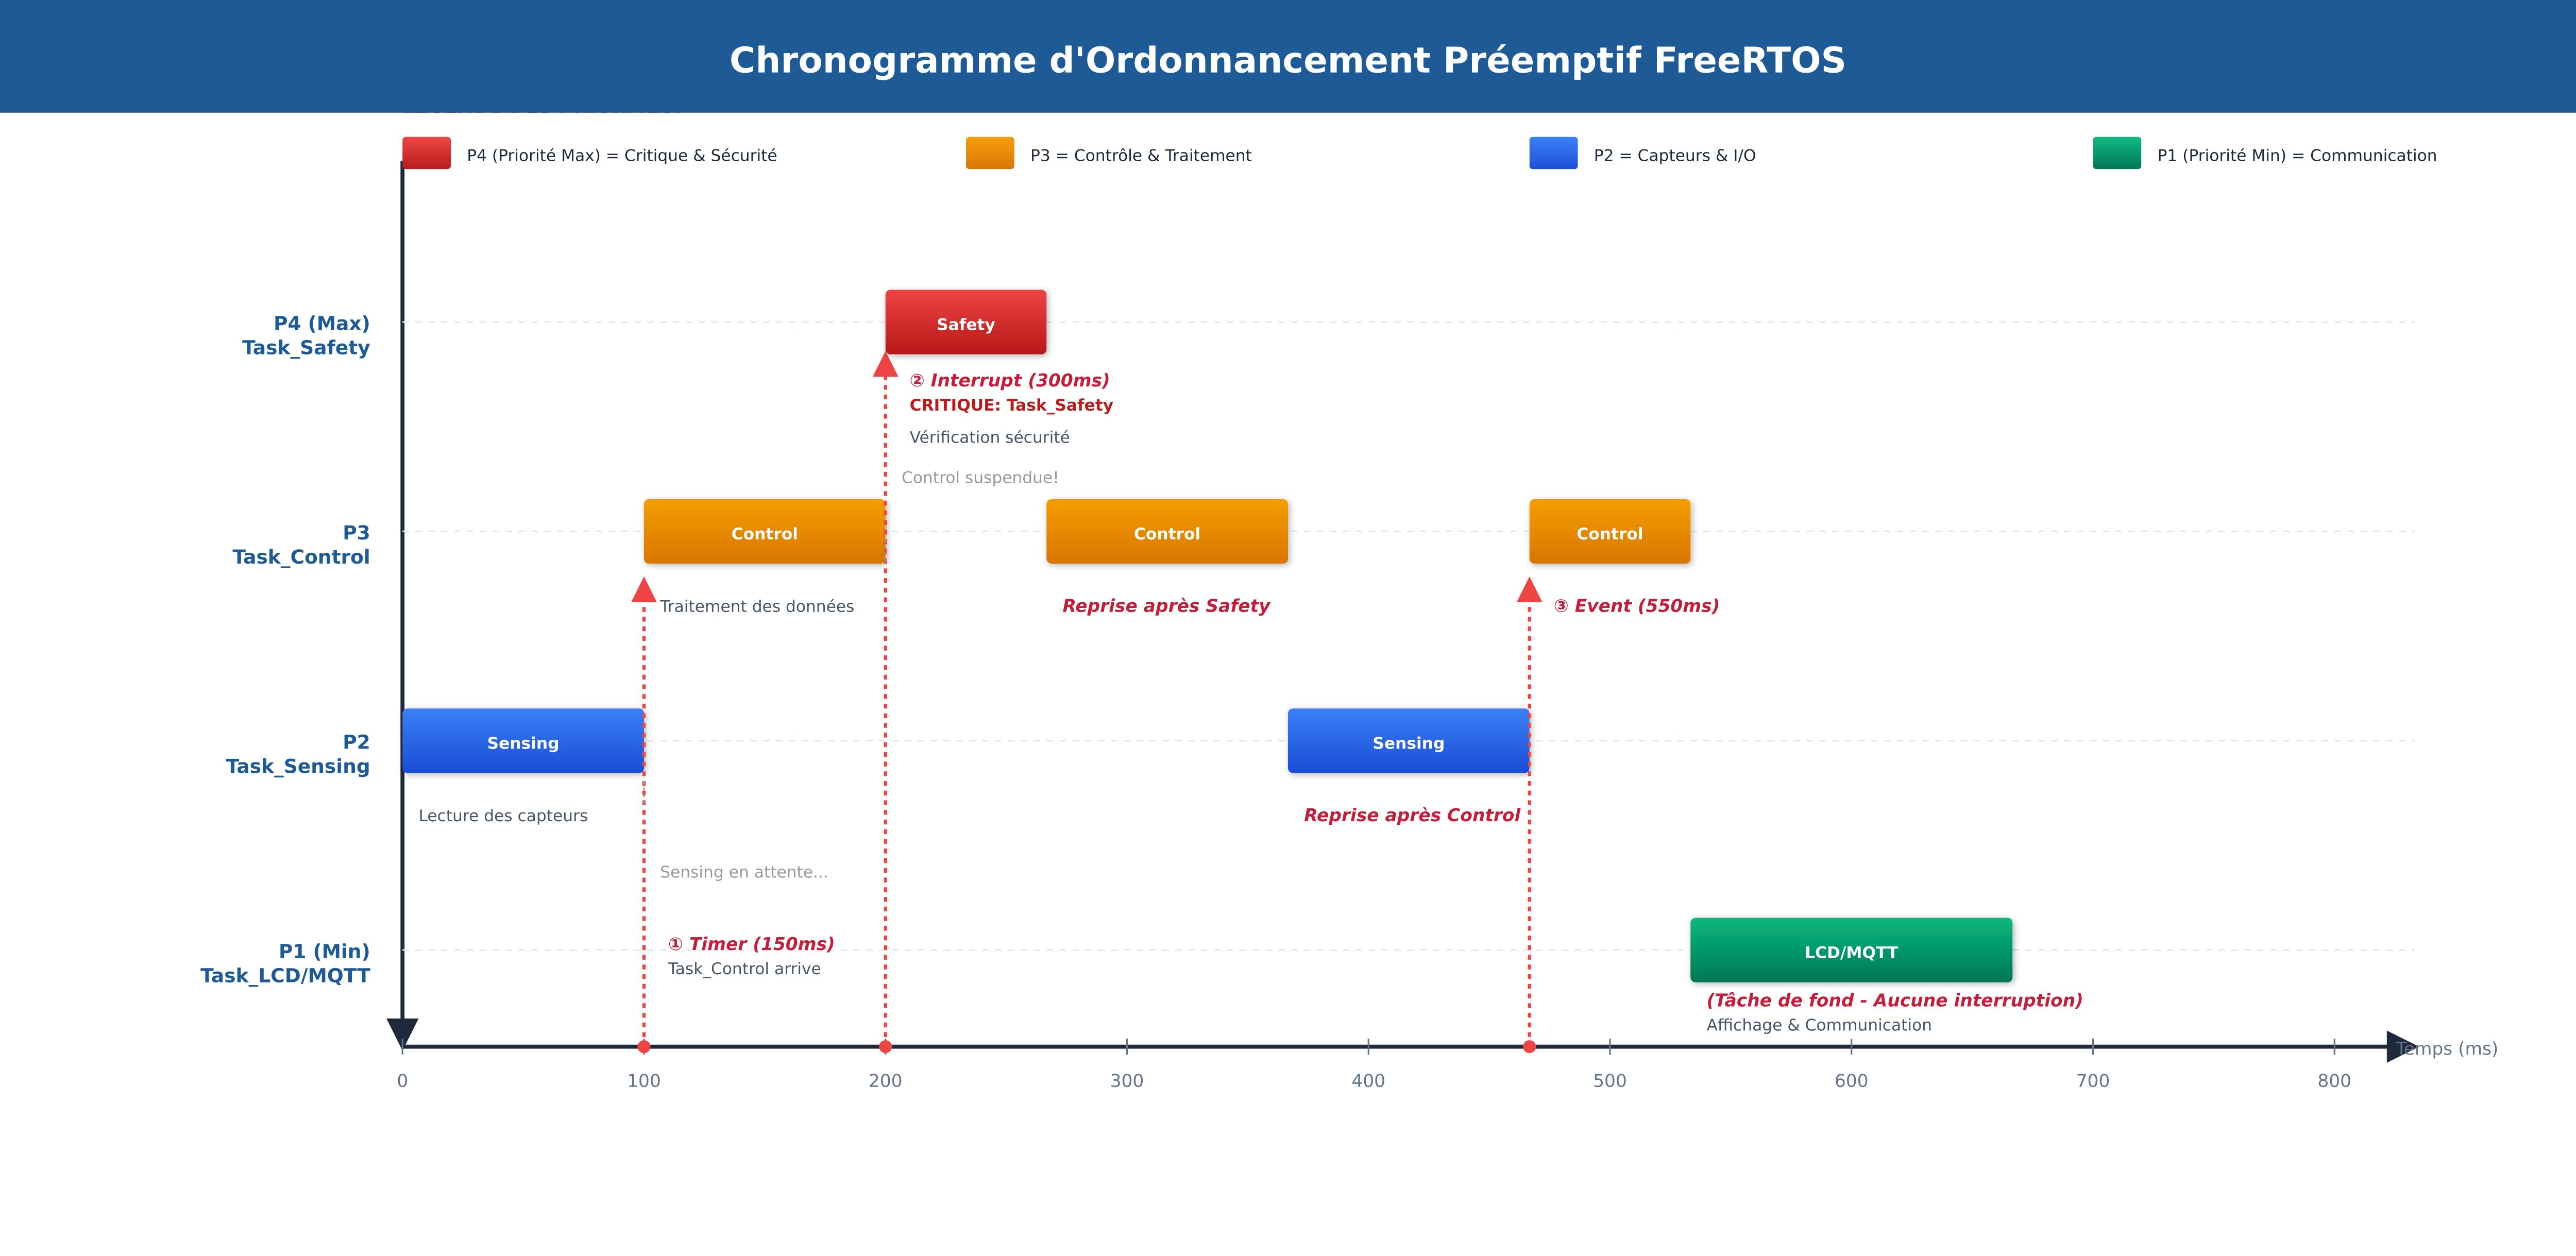
\includegraphics[width=\textwidth]{images/freertos_chronogramme.png}
    \caption{Chronogramme d'ordonnancement préemptif FreeRTOS : Illustration de la préemption et de la hiérarchie des priorités}
    \label{fig:freertos_chronogramme}
\end{figure}

L'ordonnancement repose sur trois principes fondamentaux illustrés par ce graphique :
\begin{enumerate}
    \item \textbf{La Préemption (Interruption) :} Toute tâche de priorité supérieure (ex: \textit{Task\_Safety}) suspend immédiatement l'exécution de la tâche courante (ex: \textit{Task\_Control}), garantissant une réactivité immédiate aux événements critiques.
    \item \textbf{La Reprise Automatique :} Lorsqu'une tâche prioritaire se bloque ou se termine, le noyau FreeRTOS restaure le contexte de la tâche précédemment suspendue, qui reprend exactement là où elle s'était arrêtée.
    \item \textbf{La Gestion des Priorités :} Les tâches de faible priorité (ex: \textit{Task\_LCD / Task\_MQTT}) ne s'exécutent que si aucune tâche plus prioritaire n'est prête à fonctionner, optimisant l'usage du processeur pour les fonctions vitales du système.
\end{enumerate}

\subsection{Modélisation de l'automatisme : le GRAFCET}

La complexité du cycle de traitement du soja — combinant tri mécanique, séchage thermique et pesage électronique — nécessite un outil de modélisation robuste pour garantir une exécution séquentielle sans conflit d'actionneurs. Pour ce faire, nous avons retenu le formalisme du \textbf{GRAFCET} (Graphe Fonctionnel de Commande Étape-Transition), décliné en deux niveaux d'analyse.

\subsubsection{Analyse fonctionnelle (GRAFCET niveau 1)}

Le GRAFCET de niveau 1 décrit le comportement global du système SMART-SOJA du point de vue de l'utilisateur. Le cycle se décompose en trois phases majeures :
\begin{itemize}
    \item \textbf{Phase de préparation :} Le système vérifie la disponibilité de la matière première (Trémie) et la présence d'un réceptacle (Sac) avant d'autoriser l'admission des grains.
    \item \textbf{Phase de traitement :} Elle englobe le nettoyage granulométrique par vibration, suivi d'une analyse critique de l'humidité. Si le soja dépasse le seuil de 12~\%, une séquence de séchage et de brassage est activée de manière itérative jusqu'à conformité.
    \item \textbf{Phase de clôture :} Le lot est transféré vers l'unité de pesée, les données de traçabilité sont enregistrées et le système attend le retrait du sac pour se réinitialiser.
\end{itemize}

\subsubsection{Analyse technologique (GRAFCET niveau 2)}

Le passage au niveau 2 permet de traduire les fonctions précédentes en ordres pilotables par le microcontrôleur ESP32. Cette étape définit les interfaces matérielles :
\begin{itemize}
    \item \textbf{Gestion des entrées :} Utilisation de capteurs infrarouges (IR1 et IR2) pour la détection de présence, et de sondes capacitives reliées aux convertisseurs analogique-numérique (ADC) pour l'humidité.
    \item \textbf{Pilotage des sorties :} Commande de servomoteurs par signaux PWM pour la gestion des vannes, et activation de MOSFETs de puissance pour les éléments thermiques et vibratoires.
\end{itemize}

\subsubsection{Évolutions et logique de cycle}

Pour optimiser le rendement énergétique et la qualité, l'automatisme intègre des structures algorithmiques avancées :
\begin{enumerate}
    \item \textbf{Saut de Séquence :} Si le soja est détecté comme étant déjà sec lors de l'analyse initiale, le système court-circuite l'étape de séchage pour passer directement à l'ensachage, économisant ainsi l'énergie des batteries.
    \item \textbf{Reprise de Séquence (Boucle) :} Un rebouclage est systématiquement effectué après chaque phase de séchage vers l'étape d'analyse, garantissant que seuls les grains conformes à la norme NB 01.07.004 quittent la machine.
    \item \textbf{Sûreté de fonctionnement :} Une évolution parallèle logicielle surveille en permanence le bouton d'arrêt d'urgence et les courants de fuite, capable d'interrompre le cycle à n'importe quelle étape.
\end{enumerate}

\FloatBarrier

\textbf{Double validation de l'humidité :} L'ensachage n'est autorisé que si les deux sondes Soil1 \textit{ET} Soil2 confirment individuellement $H \leq 12~\%$. Cette double validation prévient les hétérogénéités verticales du lot et les défauts de capteur isolé :
\begin{align*}
\text{Sortie\_séchage} &= (S_1 \leq 12~\%) \text{ ET } (S_2 \leq 12~\%) \\
\text{Déclenchement\_séchage} &= (S_1 > 12~\%) \text{ OU } (S_2 > 12~\%)
\end{align*}

L'ensemble de ces règles logiques et technologiques est synthétisé dans le GRAFCET de la Figure \ref{fig:grafcet_systeme}.

\begin{figure}[H]
    \centering
    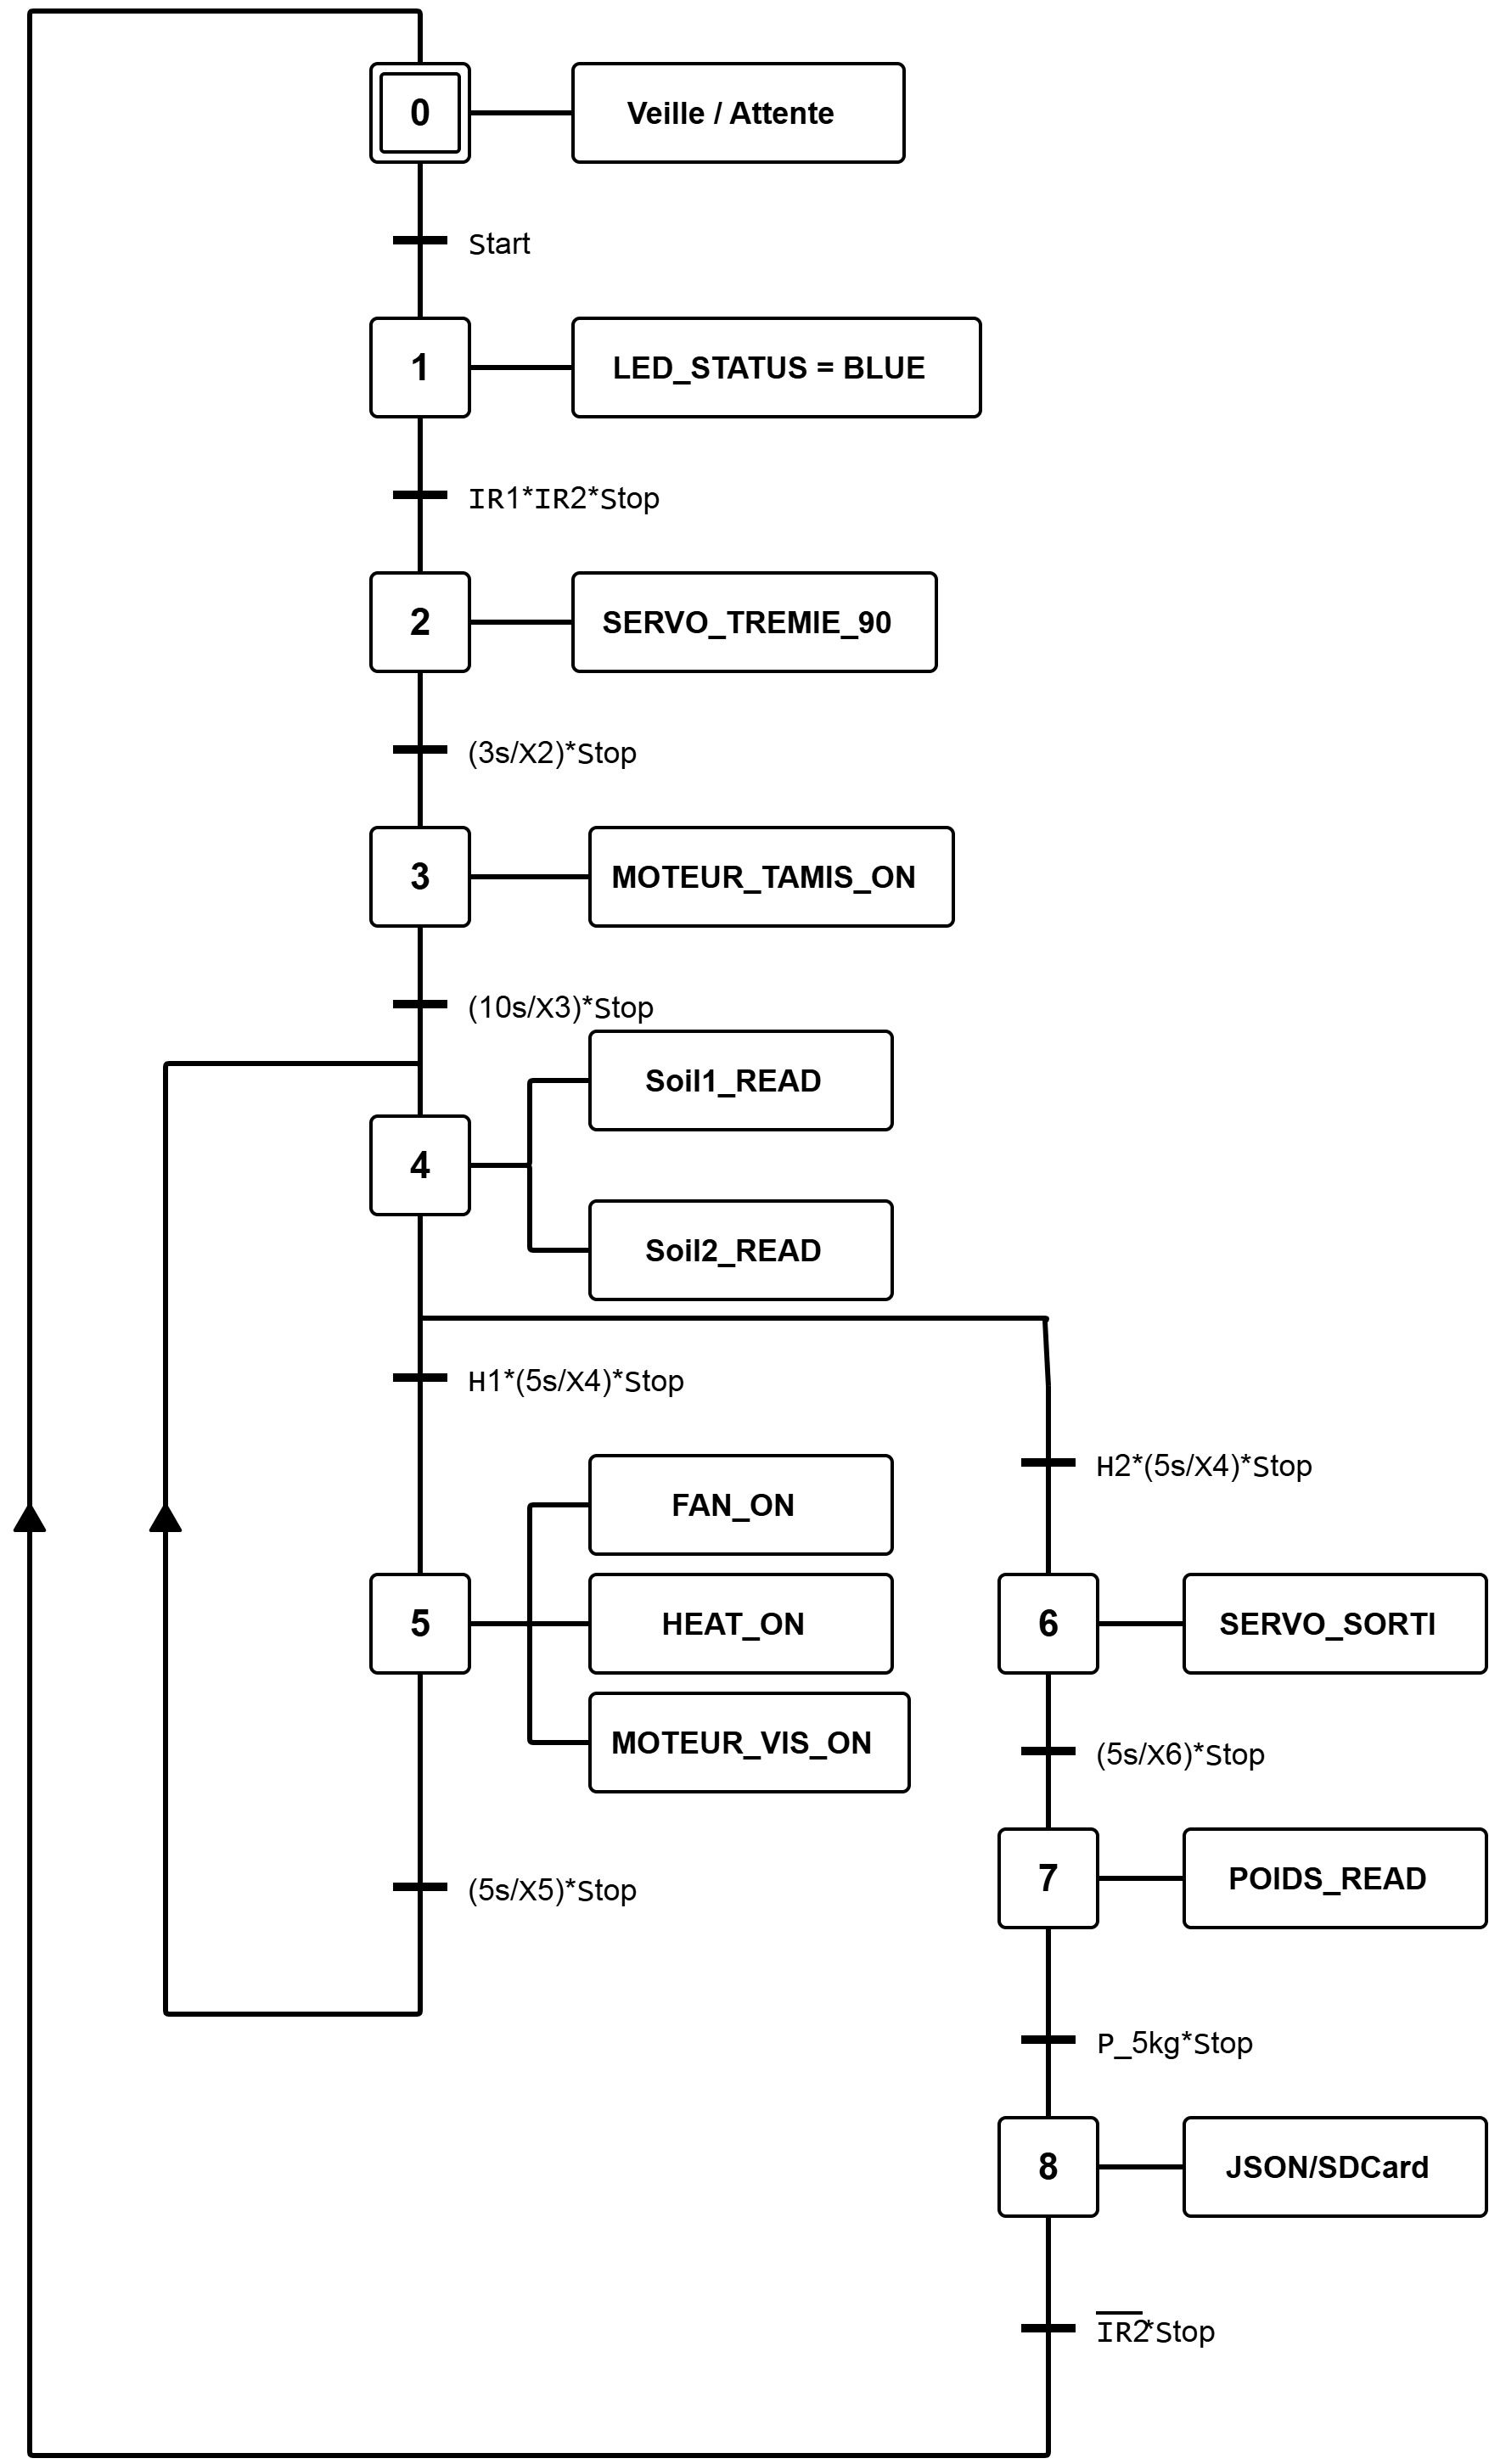
\includegraphics[width=0.6\textwidth]{images/grafcet_smart.png}
    \caption{Algorithme de contrôle séquentiel du système (GRAFCET Niveau 2)}
    \label{fig:grafcet_systeme}
\end{figure}


\subsection{Communication et traçabilité numérique}

Une fois le cycle de traitement validé par le GRAFCET, les données doivent être exportées pour assurer la traçabilité du lot. Le protocole \textbf{MQTT} (architecture Publication/Abonnement) est retenu pour sa légèreté et sa robustesse sur les réseaux à faible bande passante \cite{mqtt_org}. L'utilisation du format \textbf{JSON} garantit quant à elle l'interopérabilité des données entre l'Edge et le Cloud \cite{hanes2017}.

À chaque fin de cycle, la machine génère un \textbf{passeport numérique} au format \textbf{JSON}. Ce message regroupe l'ensemble des métriques de traçabilité (identifiant unique, horodatage, humidité moyenne et poids final) et est publié vers le broker central.

En cas de perte de connexion, ces données sont archivées sur la carte MicroSD et renvoyées dès le rétablissement du signal (\textit{Store-and-Forward}).

% Fin de la section méthodes
